\chapter{Data reliability and integrity service}
\label{cha:architecture}
This chapter presents the architecture of Data Reliability and Integrity (DRI)
service. It starts by describing the environment of VPH-Share Cloud Platform 
which specifies requirements under which DRI operates. Then it defines its 
design and interfaces with other parts of the system. At the end, the core 
validation heuristic algorithm is presented.

\section{Data and Compute Cloud Platform context}
\label{cloud-platform}
VPH-Share Data and Compute Cloud Platform project aims to design, implement,
deploy and maintain cloud storage and compute platform for application deployment
and execution. The tools and end-user services within the project will enable
researchers and medical practitioners to create and use their domain-specific
workflows on top of the Cloud and high-performance computing infrastructure.
In order to fulfill this goal, Cloud Platform will be delivered as consistent
service-based system that enables end users to deploy the basic components of
the VPH-Share application workflows (known as Atomic Services) on the available
computing resources and then enact workflows using these services.

\subsection{VPH-Share groups of users}
\label{vph-users}
VPH-Share project identifies three specific groups of users \cite{vph-deliverable-2-2}:

\begin{enumerate}
\item \textbf{Application providers} -- people responsible for developing and
installing scientific applications and software packages, typically IT experts
who collaborate with domain scientists and translate their requirements into
executable software.
\item \textbf{Domain scientists} -- actual researchers of the VPH community who
stand to benefit from access to scientific software packages provided by the 
platform. They will require the ability to access the applications in a~secure
and convenient manner via graphical interfaces provided on top of Cloud Platform.
\item \textbf{System administrators} -- priviledged users with ability to manipulate
and assign the available hardware resources to the project and define security/access
policies for other user groups. They will also make sure that the platform remains
operational by taking advantage of notification mechanisms built into the system.
\end{enumerate}

\subsection{Cloud platform architecture overview}

The general overview of Cloud Platform architecture with interactions to other parts of
the VPH-Share is illustrated in figure \ref{fig:vph-architecture}. Master UI (web portal) enables
coarse-grained invocations of the underlying core services to the specified groups of
end-users described in section \ref{vph-users}. The Cloud Platform itself will be deployed on
available cloud and physical resources.

\begin{figure}[h!]
	\centering
	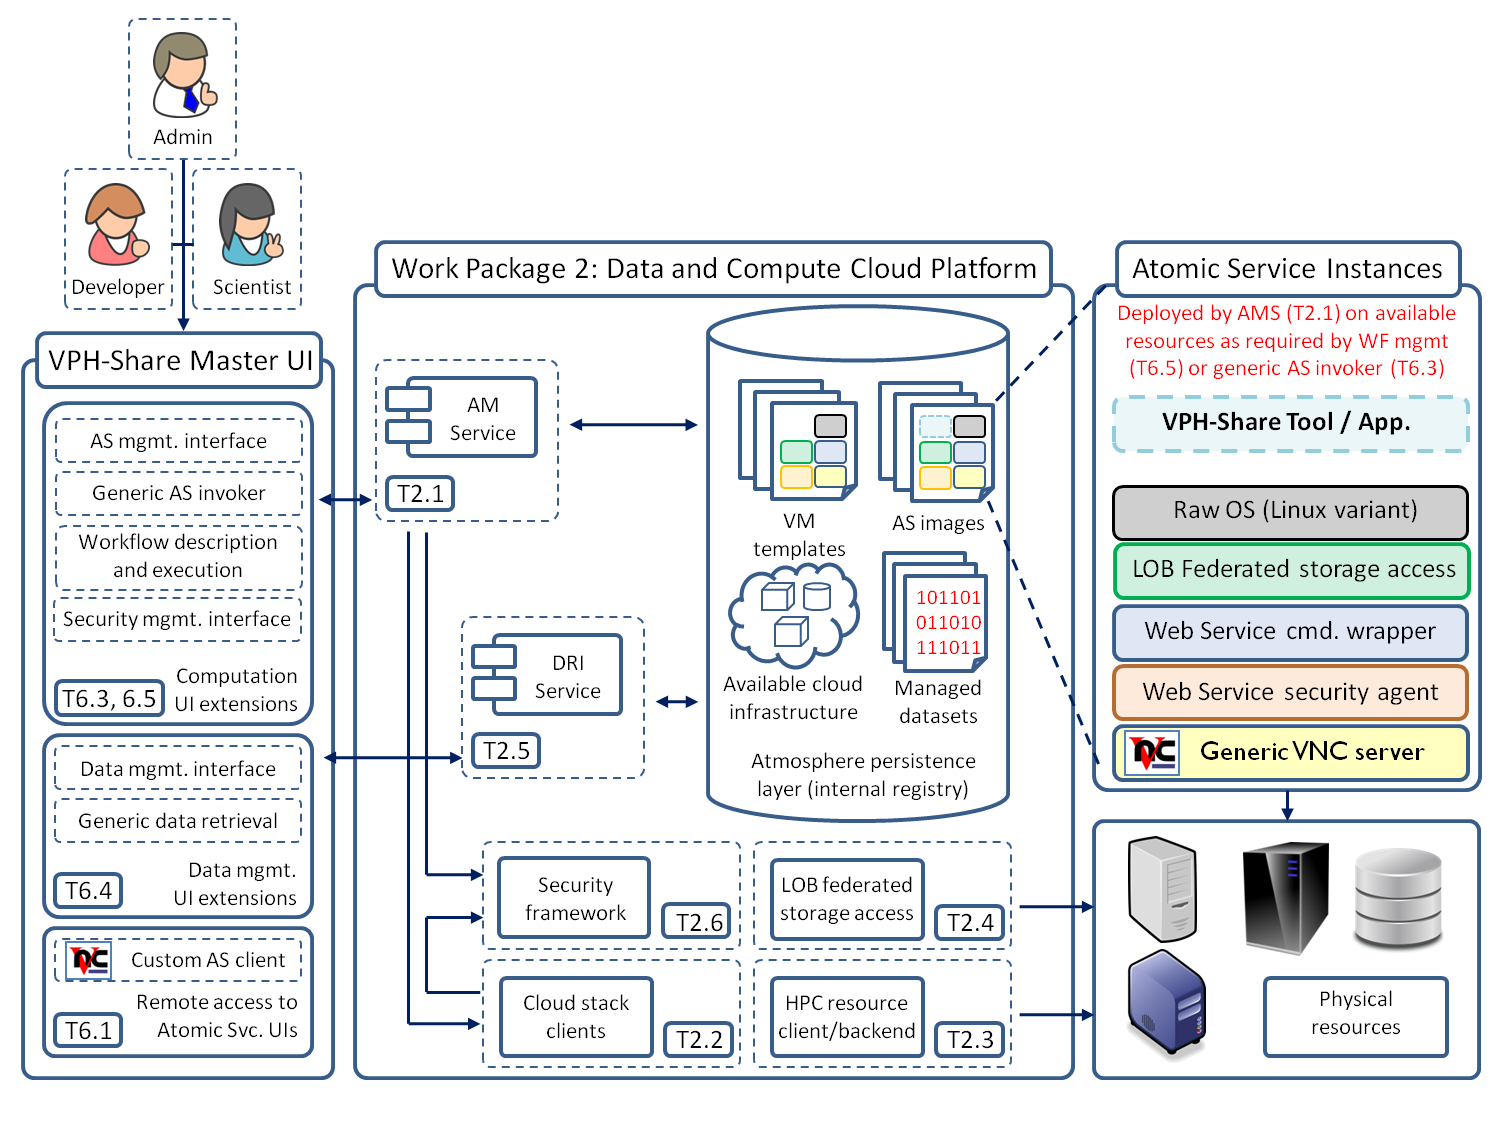
\includegraphics[width=\textwidth]{images/vph-architecture.png}
	\caption{VPH-Share Platform architecture. Specified groups of users are provided with
	functionalities of Cloud Platform through Master user interface (UI) which enables
	coarse-grained invocations of the underlying core services. Data and Compute Cloud
	Platform consists of loosly-coupled services responsible for exposing different platform
	functionalities such as federated storage access (T2.4), data integrity monitoring
	(2.5) etc. Services are deployed as Atomic Service instances (simply a~VM with add-ons).
	The platform is built on top of cloud computing resources \cite{vph-deliverable-2-2}.}
	\label{fig:vph-architecture}
\end{figure}

Cloud Platform interally consists of many loosly-coupled components deployed as Atomic Service
Instances (see section \ref{atomic-service}). Data storage is an essential functionality of
the Platform. It is achieved by
federated cloud storage which makes use of both, cloud and other storage
resources with redundancy and is accessible through common data layer --
LOBCDER service. Atmosphere Internal Registry (AIR) serves as
centralised metadata storage component which enables integration between 
loose-coupled services and is presented in subsection \ref{air}.

In VPH-Share project a strong emphasis is placed on providing data integrity,
availability and retrievability (that it can be retrieved at minimal specified
speed). To fulfill this requirement, a Data Reliability and Integrity (DRI)
service was designed, implemented and deployed as one of the core Cloud
Platform's services -- which is a primary topic of this thesis.\\

\subsection{Atmosphere Internal Registry}
\label{air}
The Atmosphere Internal Registry (hereafter also referred to as the Atmosphere
Registry, the AIR component or simply the Registry) is a core element of the 
Cloud Platform, delivering persistence capabilities. Its components and
interactions are depicted in figure \ref{fig:air-architecture}. The main 
function of AIR is to provide a technical means and an API layer for other 
components of the Cloud Platform to store and retrieve their crucial metadata. Having 
a logically centralised (though physically dispersed, if needed to meet high
availability requirements) metadata storage component is beneficial for the 
platform, as multiple elements may use it not only to preserve their “memory”,
but also to persistently exchange data. 
This is facilitated through the well-known database sharing 
model where the data storage layer serves as a means of communication between
autonomous components, making the Atmosphere Internal Registry an important 
element of the platform.

\begin{figure}[h!]
	\centering
	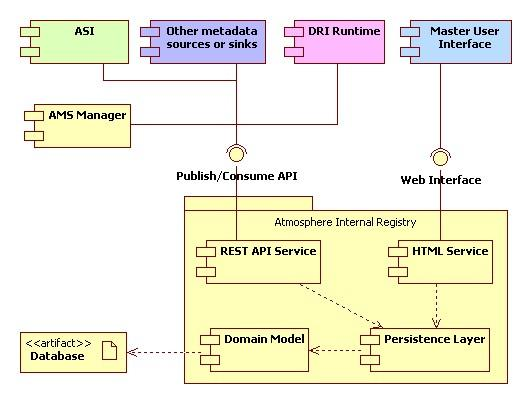
\includegraphics[width=0.7\textwidth]{images/air-architecture.png}
	\caption{The overview of Atmosphere Internal Registry (AIR) component.
	Many VPH-Share core components store and access various metadata in AIR.
	It provides REST API interface for these components, as well as web-based
	html service to enable VPH-Share users to browse the metadata via Master UI
	\cite{vph-deliverable-2-2}.}
	\label{fig:air-architecture}
\end{figure}

From DRI perspective, AIR will store necessary metadata:

\begin{itemize}
	\item \textbf{datasets metadata} and files they contain,
	\item \textbf{integrity checksums} for data validation,
	\item \textbf{service configuration}.
\end{itemize}

Such design enables us to implement DRI as stateless service.

\subsection{Federated cloud storage}
\label{federated-cloud-storage}
Data storage is an essential part of VPH-Share Cloud Platform. The increasing
popularity of cloud storage services due to high quality-cost ratio is leading
more organisations to migrate and/or adapt their IT infrastructure to operate
completely or partially in the cloud. However, as mentioned in section 2.3, 
such a solution has its limitations and implications. To overcome some of 
them one can leverage the benefits of cloud computing by using a combination 
of diverse private and public clouds. This approach is developed in Cloud
Platform as federated cloud storage, where data is stored redundantly on 
various cloud storage services. The benefits are the following:

\begin{itemize}
	\item \textbf{High availability} -- data may be temporarily unavailable 
	and/or corrupted for various reasons when system relies on a single cloud 
	storage provider, as shown in recent cases (see section 2.3). In cloud
	federation we are able to store data redundantly and switch between 
	providers when one becomes unavailable.
	\item \textbf{No vendor lock-in} -- there is currently some concern that 
	a few cloud computing providers become dominant, the so called vendor 
	lock-in issue. Migrating from one provider to another one can also be
	expensive. In cloud federation we are able to easily switch between
	providers considering their charging or policy practices.
\end{itemize}

Federated cloud storage is not sufficient to provide data unavailability 
and corruption tolerance. For this purpose, an additional service
has to be designed to actively monitor data integrity -- DRI.\\

Access to the federated cloud storage is via common access layer -- LOBCDER
service -- served by WebDAV protocol. However, DRI service will access
cloud storage services directly to take advantage of cloud federation and
to omit redundant LOBCDER overhead.

\subsection{Atomic Service}
\label{atomic-service}
In order to ensure smooth deployment for application developers, Cloud Platform
creates a~concept of Atomic Service. It can be simply described as a~VM on which
core components of the VPH-Share-specific application software have been installed,
wrapped as a~virtual system image and registered for usage within the platform. The
process of creating new atomic service is depicted in figure \ref{fig:atomic-service}.
Typical application software installations provided by Atomic Service is federated
storage access, web service command wrapper and web service security agent. Additionally,
Cloud Platform takes care of instantiating various Atomic Services. Atomic Service
Instance is a~specific atomic service deployed on computing resources and providing
VPH-Share application functionality through a~web service (SOAP or REST) interface.\\

Services providing core functionality within VPH-Share will be also deployed as atomic
service instances. 

\begin{figure}[h!]
	\centering
	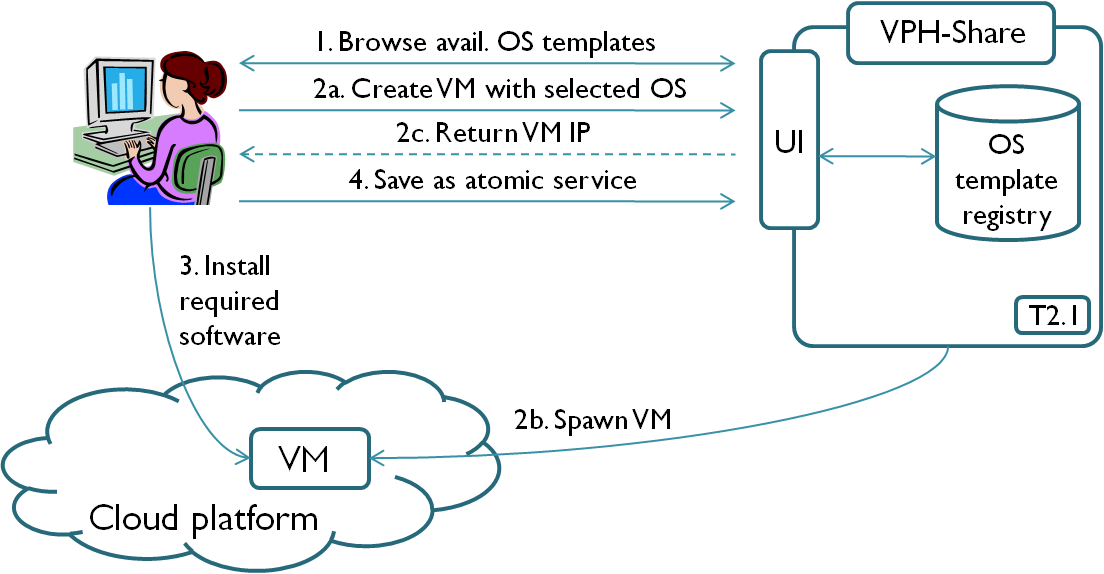
\includegraphics[width=0.8\textwidth]{images/vph-atomic-service.png}
	\caption{The process of creating and instatiating new Atomic Service
	\cite{vph-deliverable-2-2}.}
	\label{fig:atomic-service}
\end{figure}


\section{DRI data model}
The Cloud Platform concerns itself primarily with access to binary data, 
especially via file-based interface. Managed dataset represents a single entity
that can be managed. At its core, it consists of a~selection of
files, to which a portion of metadata is appended and stored in AIR reigstry. 
As data integrity is a crucial requirement of the platform, the datasets can be
tagged for automatic data integrity monitoring (DRI). 

\begin{figure}[h!]
	\centering
	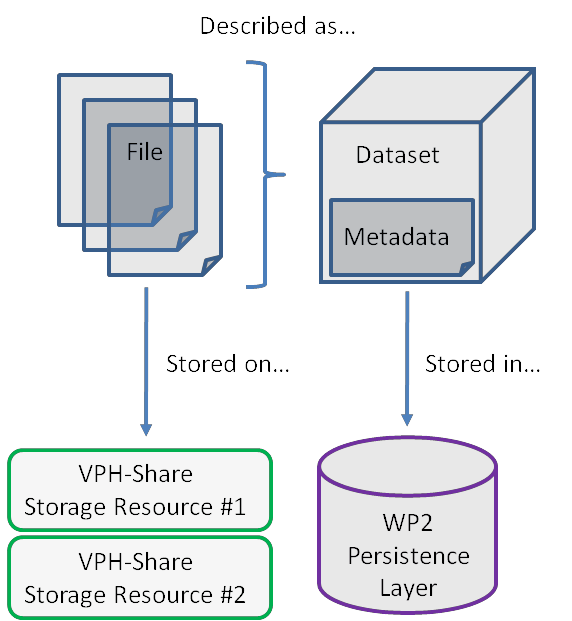
\includegraphics[width=0.5\textwidth]{images/managed-dataset.png}
	\caption{Schematic representation of VPH-Share managed dataset. Managed
	dataset consists of an arbitrary number of files (logical data) that are stored
	on one or more storage resources. The metadata regarding managed dataset is persisted
	in AIR \cite{vph-deliverable-2-2}.}
	\label{fig:managed-dataset}
\end{figure}

\subsection{Metadata schema}
Each managed dataset may consist of an arbitrary number of files (logical 
data) and can be stored on one or more storage resources (data source).
Specific security constraints can be attached to data items, i.e. it cannot be
used in public clouds. In DRI component, validation checks are of configurable
policy (management policy). The schema is depicted in the figure 
\ref{fig:data-model}.\\

\begin{figure}[h!]
	\centering
	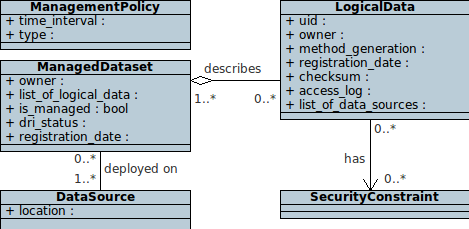
\includegraphics[width=0.8\textwidth]{images/data-model.png}
	\caption{DRI service metadata schema. It generally reflects the concept of
	managed dataset presented in figure \ref{fig:managed-dataset}. Managed dataset
	consists of arbitrary number of logical data and is deployed on one or more
	data sources. Logical data can have security contraints attached to it. Additionally,
	a management policy can be attached to every managed dataset.}
	\label{fig:data-model}
\end{figure}

The managed dataset metadata consists of the following elements:

\begin{itemize}
	\item \textbf{owner} -- reference to user ID of dataset creator,
	\item \textbf{list of logical data} -- list of logical data ids it consists of,
	\item \textbf{is managed} -- marker determining whether dataset's integrity
	is monitored,
	\item \textbf{DRI status} -- dataset's reliability and integrity status,
	\item \textbf{date of registration}.
\end{itemize}

\noindent
Additionally, each logical data will consist of the following attributes:

\begin{itemize}
	\item \textbf{owner} -- reference to user ID,
	\item \textbf{method of generation} -- whether it was uploaded manually, 
	generated by an application or registered externally,
	\item \textbf{date of registration}
	\item \textbf{checksum} -- file's value of a cryptographic hash function
	calculated upon registration and used to validate integrity and 
	availability of file,
	\item \textbf{list of data sources} -- to which the file is currently
	deployed,
	\item \textbf{access log}.
\end{itemize}

While this schema is expected to cover all the requirements addressed in the
DRI service, we foresee that additional metadata can be added later without
affecting already stored.

\subsection{Tagging datasets}
Before automatic verification of managed datasets can take place, it is first
necessary to tag specific data as subject for management. It is foreseen that
the DRI component will involve a user interface extension (portlet-based) to
enable authorised users to tag specific datasets for automatic management. This
interaface will display the existing data storage resources and allow creation
of new managed datasets consisting of selected files.\\

In addition to UI based tagging, the DRI component provides API-level access
for the same purpose, whenever a VPH-Share application (or workflow) needs to
tag specific data as a managed dataset.

\section{Architecture}
The DRI Runtime is responsible for enforcing data management policies. It keeps
track of managed components and periodically verifies the accessibility and
integrity of the managed data. It operates autonomously as well as on request.
It also interacts and cooperates with the other important Cloud Platform's
components (see section \ref{cloud-platform}) to fulfill its goal. At the core
of the service is an application that periodically polls the AIR registry for
a~list of managed datasets and then proceeds to verify the following:

\begin{itemize}
	\item the availability of each dataset at locations read from the AIR
	registry,
	\item the binary integrity of each dataset (checksum-based validation).
\end{itemize}

The DRI Runtime contacts individual data sources and validates the integrity
and availability of the data stored on these resources. Should errors occur,
the DRI Runtime invokes a notification service to issue a warning message
to subscribed system administrators (typically, the user defined as the 
dataset's owner).\\

\subsection{Overview}
The architecture of the DRI service was mostly influenced by the Cloud Platform
environment (section \ref{cloud-platform}) and the requirements and challenges
it introduces (section \ref{requirements}). Figure \ref{fig:dri-architecture}
presents its overview.\\

\begin{figure}[h!]
	\centering
	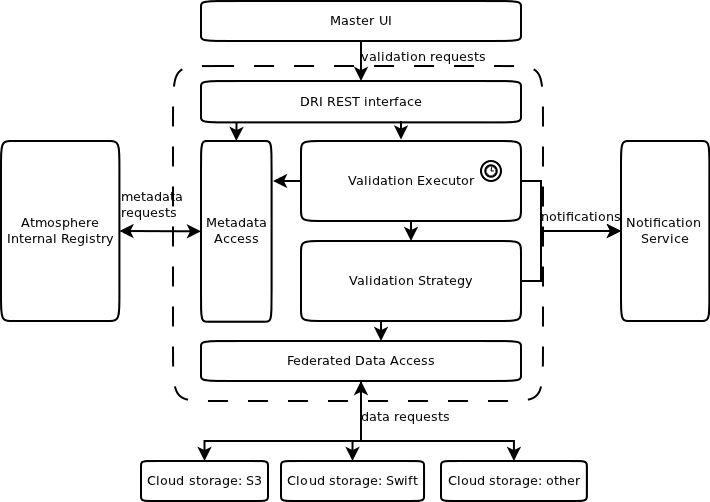
\includegraphics[width=0.8\textwidth]{images/dri-architecture.png}
	\caption{DRI architecture overview. It exposes REST API interface for other
	Cloud Platform components, mostly Master UI. The design is divided into
	modules that are responsible for providing separate functionality.
	ValidationExecution module is responsible for periodical as well as on-request
	based validation of datasets. All of the integrity metadata is provided
	through MetadataAccess module. The complexity of accessing different cloud
	storage providers is abstracted with FederatedDataAccess layer.}
	\label{fig:dri-architecture}
\end{figure}

The DRI Runtime consists of a couple of subcomponents which interact with each
other as well as with other services described. It exposes REST service
interface to be invoked by Master UI or the Atomic Services (see subsection
\ref{dri-interface} for details). MetadataAccess component is responsible for
retrieving necessary metadata from the AIR registry. Access to the federated
cloud storage is performed via FederatedDataAccess layer in order to hide
the underlying complexity and differences between various cloud storage access.
ValidationExecutor represents the core of the DRI. Its objective is to manage
all the validation tasks, both periodical and requested by user. For
each logical data it invokes ValidationStrategy component to perform
its data validation algorithm.

\subsection{Interface and API}
\label{dri-interface}
As hinted upon in the preceding sections, DRI provides end-user interfaces
in the form of a~Master UI portlet, as well as an API implemented by the
Runtime service, where DRI features may be invoked directly by other VPH-Share
intrastructure components.\\

Here we intend to focus on the API, which provides access to the low-level
functionality of DRI and enables it to be configured.\\

As DRI exposes a stateless Web Service, all configuration parameters are stored
in the Atmosphere Internal Registry. Whenever a~configuration change request
is invoked the DRI automatically updates policies stored in AIR. In light
of this, the DRI API supports the following operations:

\begin{itemize}
	\item \textbf{\textit{getDataSources(): DataSourceID[]}} --
	returns a list of currently registered data storage resource identifiers;
	
	\item \textbf{\textit{getDataSource(dataSourceID):
	DataSourceDescription}} -- returns the information on a specific storage
	resource, as stored in the Atmosphere Internal Registry in a form of XML
	document describing the structure of storage resource;
	
	\item \textbf{\textit{registerManagedDataset(DatasetDescription) :
	datasetID}} -- tags a new dataset for management given in
	the form XML document describing the structure of the dataset;
	
	\item \textbf{\textit{alterManagedDataset(DatasetID, DatasetDescription) :
	void}} -- changes the dataset specification stored in the AIR. This action
	should be used to add or remove files from a~managed dataset;
	
	\item \textbf{\textit{removeManagedDataset(DatasetID) : void}} -- excludes
	the specified dataset from automatic management. This does not delete the
	data, it merely stops DRI Runtime from monitoring them;
	
	\item \textbf{\textit{getManagedDataset(DatasetID) :
	ManagedDatasetDescription}} -- requests information on a specific managed
	dataset stored in the AIR, returning XML document specifing the structure
	of the managed dataset;
	
	\item \textbf{\textit{getOwnerManagedDataset(User) : DatasetID[]}} --
	returns a list of user's managed dataset ids;
	
	\item \textbf{\textit{assignDatasetToResource(DatasetID, 
	DataSourceeID) : void}} -- requests DRI to monitor the availability of
	a specific managed dataset in a specific storage resource. If this dataset
	is not yet present on the requested storage resource, it will be
	automatically replicated there;
	
	\item \textbf{\textit{unassignDatasetFromResource(DatasetID, 
	StorageResourceID) : void}} -- requests DRI to stop monitoring the 
	availability of a specific managed dataset on a specific storage resource.
	If the dataset is not present on the selected storage resource, this action
	has no effect;
	
	\item \textbf{\textit{validateManagedDataset(DatasetID) : output}} --
	performs asynchronous validation of the specific dataset and produces a
	document which lists any problems encountered with the dataset's
	availability on the storage resources to which it had been assigned;
	
	\item \textbf{\textit{setManagementPolicy(ManagementPolicy) : void}} --
	changes monitoring parameters. ManagementPolicy is an XML document
	specifying the frequency and type of availability checks performed on
	managed datasets;
	
	\item \textbf{\textit{getManagementPolicy() : ManagementPolicy}} --
	retrieves an XML description of the management policy.
\end{itemize}

\begin{figure}[h!]
	\centering
	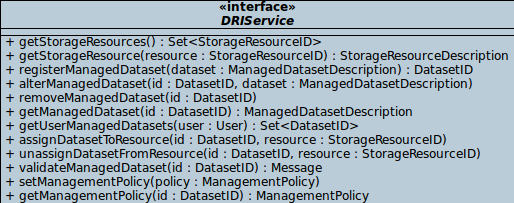
\includegraphics[width=\textwidth]{images/dri-interface.png}
	\caption{DRI Service interface. It provides flexible set of methods to
	manipulate integrity monitoring of datasets.}
	\label{fig:dri-interface}
\end{figure}

Each invocation requires to be augmented by the security token which can be
intercepted and parsed by the security component residing on the virtual
machine on which the DRI Runtime operates.

		\subsection{Typical use cases execution flow}
The two main tasks performed by the DRI is monitoring of data integrity and
replication of managed datasets among various data sources. Now, we will
present a typical execution flow for this tasks through DRI subcomponents
presented in figure \ref{fig:dri-architecture} using sequence diagrams.\\

We start with data validation illustrated in figure
\ref{fig:validation-diagram}. The \textit{validateManagedDataset()} method is the one
designed to be called by the user, however, the incorporated logic for periodic
integrity checks is the same, as ValidationExecutor fetches all the managed
datasets from AIR and invokes this operation for each of them.\\

\begin{figure}[h!]
	\centering
	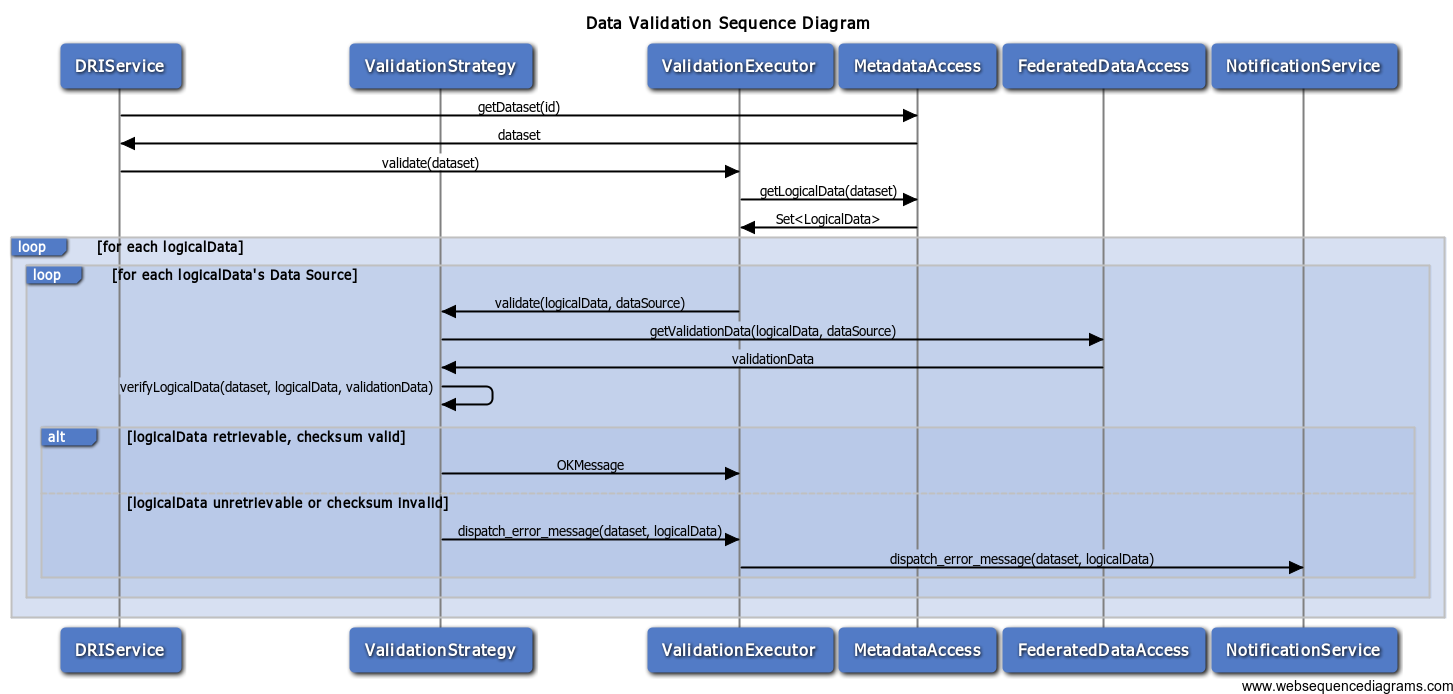
\includegraphics[width=\textwidth]{images/validation-diagram.png}
	\caption{DRI \textit{validateManagedDataset()} call sequence diagram}
	\label{fig:validation-diagram}
\end{figure}

Upon \textit{validateManagedDataset()} call, the DRI service retrieves dataset's
metadata from AIR registry invoking \textit{getDataset(id)} on MetadataAccess object
and passes it to the ValidationExecutor to apply data availability and
integrity check. Subsequently, ValidationExecutor retrieves the metadata of
all the logical data items which are part of the specified dataset invoking
\textit{getLogicalData(dataset)} on MetadataAccess. Validation occurs separately for
each logical data and against every data source on which it is stored by
ValidationStrategy object which implements efficient validation protocol. To
perform this operation, it has to get some necessary portion of data from data
source by calling \textit{getValidationData(logicalData, dataSource)} on
FederatedDataAccess object. With this necessary data, ValidationStrategy can
verify whether the specified logical data is available and valid. If not, the
error message is dispatched via NotificationService. It incorporates all or
nothing strategy, which means that the corruption of a single logical data
results in marking whole dataset as invalid. However, detailed error message
informs which items' corruption has been detected on which data sources. The
\textit{validateManagedDataset()} call performs asynchronously (no return value), but
the result of the operation can be checked via NotificationService.\\

\begin{figure}[h!]
	\centering
	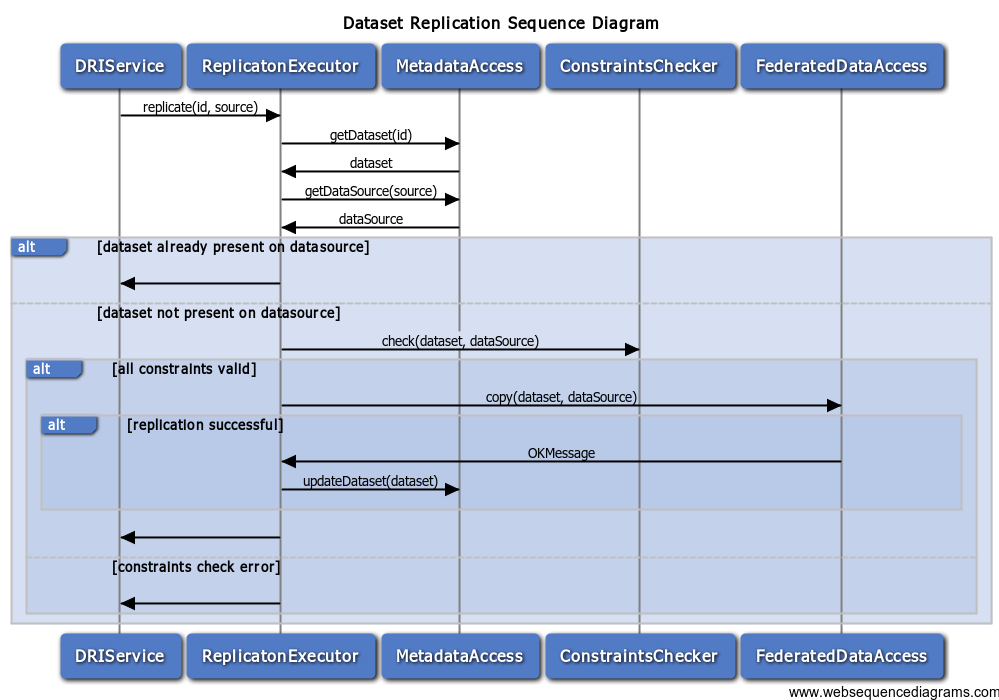
\includegraphics[width=\textwidth]{images/replication-diagram.png}
	\caption{DRI \textit{assignDatasetToResource()} call sequence diagram}
	\label{fig:replication-diagram}
\end{figure}

Upon \textit{assignDatasetToResource()} 
call (figure \ref{fig:replication-diagram}), the DRIService retrieves
dataset's and data source's metadata from AIR registry invoking
\textit{getDataset(id)} and \textit{getDataSource(source)} on MetadataAccess object and
passes it to the ReplicationExecutor. If dataset is already present on the
specified location, this operation has no effect. Subsequently,
ReplicationExecutor checks all the constraints, via 
\textit{check(dataset, dataSource)} call, that may be associated with the
dataset (such as it cannot be stored in public clouds) and if they are valid,
it performs the replication. This operation simply copies data from one data
source on which the dataset is already present to the specified data source.
In case of any failures, the operation aborts with no side effects. Upon
successful execution, the necessary dataset metadata is updated in AIR registry
(\textit{updateDataset(dataset)} call).\\

	\section{Data validation mechanism}
	\label{section:validation-algorithm}
At the heart of DRI service lies its validation heuristic algorithm which is
going to be described now in detail. As it was discussed in chapter 
\ref{cha:state_of_the_art}, a lot of 
effort was put into ensuring data integrity and availability on storage
resources. However, cloud storage model sets new challenges in this area due to
its constraints and limitations presented in section 2.3. The problem was
addressed in the papers described in section 2.4, one of which - Proofs of
Retrievability - became the basis for many enhancements, modifications and
improvements. Each of the solution approaches difficulties with vast amount of
data stored on cloud storages by creating sophisticated protocols which download
only a fraction of data $(1-10\%)$ and try to guarantee possibly the highest
error-detection rate. Unfortunately, introduced solutions do not address
performance issues of these protocols with regard to typical cloud storage
interfaces and VPH-Share platform requirements:

\begin{itemize}
	\item requesting many small fragments of data greatly affects network
	overhead as each fragment requires separate HTTP request,
	\item cloud storages do not allow executing users' code,
	\item VPH-Share platform requires storing data in unmodified form.
\end{itemize}

These limitations make these solutions impractical. For the needs of DRI
service, a~new approach was designed with practical feasibility and low network
overhead as main objectives in mind. Our heuristic utilizes spot-checking
technique to verify data integrity with high
probability. Unlike cited mechanisms \cite{dip, por} which generally implement
fine-grained spot-checking, we are aware of cloud storage limitations and
employ coarse-grained spot-checking, realizing that it will result in reduced
error-detection rate.

		\subsection{Algorithm description}
According to the data model described in section 3.1, dataset is a set of files
stored on cloud storage resource. To be able to validate dataset's integrity,
it is firstly necessary to retrieve dataset's data, then compute and store some
checksum metadata for each file. During the validation process, the dataset's
data is retrieved and checksums are computed again to compare them with the
original ones. The algorithm 1 illustrates the pseudocode
of this operation.\\

\begin{figure}
\begin{algorithm}[H]
	\SetLine
	\linesnumbered
	\KwData{valid dataset $id$}
	\KwResult{true if dataset valid, error messages otherwise}
	dataset $=$ get$\_$dataset$\_$metadata(id)\;
	files $=$ get$\_$dataset$\_$files(dataset)\;
	\For{file in files}{
		\For{data$\_$source in dataset.get$\_$data$\_$sources()}{
			data $=$ get$\_$validation$\_$data(file, data$\_$source)\;
			\If{data $== null$}{
				dispatch$\_$error$\_$message(file, data$\_$source)\;
			}
			result $=$ validate$\_$data(data, file, dataset)\;
			\If{result is invalid}{
				dispatch$\_$error$\_$message(file, data$\_$source)\;
			}
		}
	}
\caption{Dataset validation algorithm}
\end{algorithm}
\label{fig:algorithm-pseudocode}
\end{figure}

To validate a dataset, the metadata of it and all the files it consists of
have to be retrieved (lines 1--2). Then, each file is validated against every
data source it is stored on (lines 3--4). To validate a single file, the
algorithm retrieves its necessary data (line 5). If errors occur, the file's
unavailability message is reported (lines 6--8). Otherwise, integrity checksum
is computed and checked with the original one (line 9). Any resulting integrity
error is reported (lines 10--12).\\

The core part of the validation mechanism is the validation algorithm
(validation protocol) which prepares dataset's metadata and then is able to
validate it. As a typical integrity checking algorithm it comprises of two 
phases: 

\begin{enumerate}
	\item \textbf{setup} -- takes place once (or after each file update) and 
	generates checksum used during every validation phase. During this
	phase the file is divided into $n$ chunks of size $F \over n$ (where $F$
	denotes the size of entire file) and MAC hash is computed for every data
	chunk. Then, a set of $n$ checksums is stored in metadata registry for
	further use.
	\item \textbf{validation} -- takes place on every dataset validation 
	request. During this phase, the file is again divided into $n$ chunks of size $F \over n$ and
	pseudorandom number generator selects $k$ out of $n$ chunk indexes that are
	downloaded and their checksums computed. Then, computed checksums are
	compared with original ones stored in metadata registry.
\end{enumerate}

These phases are graphically presented in figure \ref{fig:algorithm-scheme}.\\

\begin{figure}
	\begin{subfigure}[h!]{0.45\textwidth}
		\centering
		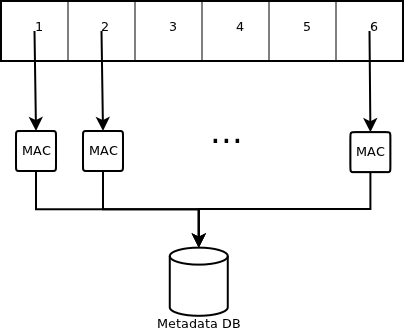
\includegraphics[width=\textwidth]{images/algorithm-setup.png}
		\label{fig:setup}
		\caption{Setup phase}
	\end{subfigure}
	\begin{subfigure}[h!]{0.45\textwidth}
		\centering
		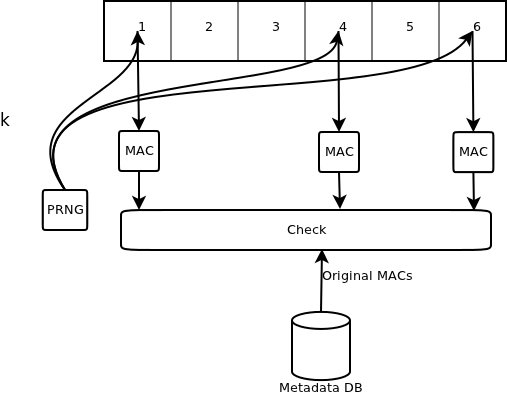
\includegraphics[width=\textwidth]{images/algorithm-validation.png}
		\label{fig:validation}
		\caption{Validation phase}
	\end{subfigure}
	\caption{Single file validation heuristic consists of two phases: setup
	and validation. In setup phase (a), the file is divided into $n$ chunks and
	MAC hash is computed for every data chunk which is then stored in metadata
	registry. In validation phase (b), the file is again divided into $n$
	chunks and pseudorandom number generator selects a set of $k$ out of $n$
	chunk indexes that are downloaded, their checksums computed and compared
	with the original ones stored in metadata registry.}
	\label{fig:algorithm-scheme}
\end{figure}

Values $k$ and $n$ are configurable and can be set to fulfill specified 
requirements. The greater the value of $n$, the smaller the chunks are (see
setup phase description) and more separate $k$ HTTP requests need to be sent to
maintain demanded error-detection rate. With fixed $n$, the greater the value
of $k$, the higher error-detection rate.\\

Datasets consisting of large number of small files can lead to the performance 
bottleneck for two reasons: many separate HTTP requests for each small file and
big storage overhead as chunks are small for small files, but for each a MAC
checksum is stored. For this reason, one additional parameter $threshold$ was 
introduced to improve performance over small files. Data integrity for files
of size smaller than $threshold$ is provided by classic entire-file SHA-256 
checksum. The value of $threshold$ parameter will be established empirically
based on performance test results presented in chapter \ref{cha:testing}.

\subsection{Algorithm analysis}
\label{algorithm-analysis}
Validation algorithm described in the previous subsection is rather simple in 
its design, but poses properties that make it practically feasible:

\begin{itemize}
	\item files are stored in unmodified form,
	\item network overhead and number of HTTP requests can be configured by 
	$n$ and $k$ parameters,
	\item error-detection rate can be configured by $n$ and $k$ parameters.
\end{itemize}

Detailed algorithm description enables theoretical estimation of the most
interesting properties that characterize our solution:

\begin{itemize}

\item \textbf{Error-detection rate} -- expresses the probability to detect data
corruption. For small changes, its value is equal to the probability that the
change took place within the $k$ blocks that are verified:

\begin{equation}
	E_{det} = {k \over n} \hspace{0.6cm} \ for\ small\ changes.
\end{equation}

However, if the prover has modified or deleted substantial $e$-portion of $F$,
then with high probability, it also changed roughly an $e$-fraction of
chunks.

\item \textbf{Network overhead} -- expresses the fraction of data that has to
be retrieved in order to verify the integrity on desired level. As in our
scheme, we download $k$ out of $n$ chunks (each of size $F \over n$), the
network overhead value is proportional to:

\begin{equation}
	N_{over} \sim F \times {k \over n}.
\end{equation}

\item \textbf {Execution time} -- expresses the time needed to validate a file
of size $F$. It depends on average network download speed, as well as on
network latency to the cloud provider. Each HTTP request introduces latency, so
the more requests are sent, the more network efficiency is affected. We
estimate this value in the following way: each chunk
of size $F \over n$ is downloaded in $F \over {n \times speed}$ time (where
$speed$ is download speed in bits/s) plus additional request latency time. As
we validate $k$ chunks per validation phase, we get the execution time: 

\begin{equation}
	T_{exec} \sim k \times ({F \over {n \times speed}} + latency) 
\end{equation}

However, the latency factor can be drastically reduced by performing a set of
HTTP requests concurrently.

\end{itemize}

\begin{table}[h!]
\centering
\begin{tabular}{|l||c|c|}
	\hline
	Metric     & our approach                                           & whole-file approach \\ \hline \hline
	$E_{det}$  & ${k \over n}$                                          & 1 \\ \hline
	$N_{over}$ & $\sim F \times {k \over n}$                            & $\sim F$ \\ \hline
	$T_{exec}$ & $\sim k \times ({F \over {n \times speed}} + latency)$ & $\sim {F \over speed} + latency$ \\ \hline
\end{tabular}
\caption{Performance metrics comparison between our and whole-file approaches}
\label{tab:metrics-comparison}
\end{table}

In table \ref{tab:metrics-comparison} we summarize the three metrics values
for our approach in comparison with whole-file validation approach. Practical
performance evaluation with varying values of the parameters $n$, $k$ and
$threshold$) and in the real cloud storage environment is presented in chapter
\ref{cha:testing}.

\section{Summary}
This chapter presented in-depth the design and architecture of data reliability and
integrity (DRI) service. The architecture of the VPH-Share Cloud Platform was introduced
to provide a~context in which DRI is developed and that mostly influenced its requirements.
Given that, we determined the DRI data model and formulated its -- functional and non-functional
-- requirements. The API of the service tries to reflect all of the identified use cases.\\

At the end, we presented the design of the network efficient algorithm that
tries to take cloud storage limitations into account and provide means of network efficient
corruption detection on some level of probability. The concept is based on POR and DIP schemes presented in section
\ref{cloud-integrity-approaches}. Finally, we presented the equations describing the algorithm features.

